
\documentclass[11pt]{amsbook}
\usepackage[turkish]{babel}

\usepackage{../Ceyhun}	% ------------------------
\usepackage{../amsTurkish}


\usepackage{lipsum}



\begin{document}

% ++++++++++++++++++++++++++++++++++++++
\hPage{2}
% ++++++++++++++++++++++++++++++++++++++
% =======================================

Tanım 1.1.1 de olduğu gibi tanımlanan her \emph{soyut} çizgeye ilişkin, \emph{somut} bir \emph{çizimsel gösterimin} varolacağı gözden kaçmamalıdır. 
% I don't know the reference of that definition because it is not in my page. Therefore I wrote it by hand, instead of \ref{def:...}.
Örneğin, $$\Psi = (a_1,a_2,a_3,a_4,a_5)$$ ve $$\Delta = (d_1,d_2,d_3,d_4)$$ kümeleri arasındaki çakışım ilişkisi,
 $$ a_1 \rightarrow (d_1,d_2)$$ $$ a_2 \rightarrow (d_1,d_3)$$ $$ a_3 \rightarrow (d_1,d_4)$$ $$ a_4 \rightarrow (d_2,d_4)$$ 
$$ a_5 \rightarrow (d_3,d_4)$$ olsun. Bu soyut Ç(4,5) çizgesinin, somut çizimsel gösterimi \reffig{fig:1.1.1} de verildiği gibi bulunabilir.
\begin{figure}[htb]
	\centering
	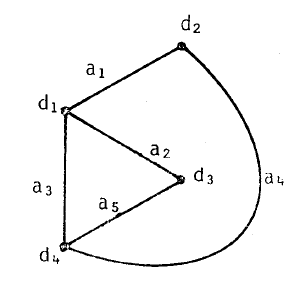
\includegraphics[width=0.45\textwidth]{images/ceyhun-002-fig01}
	\caption{Ç(4,5) Çizgesinin çizimsel gösterimi.}
	\label{fig:1.1.1}
\end{figure}

\end{document}  


